\clearpage
\section{Automated Judge Robustness and Adjudication Sensitivity}\label{app:judge_robustness}
\paragraph{Archived cross-model reassessment.} We audited an author-supplied post-freeze reassessment configured as \texttt{gemini-3.8-flash} through relay serving (temperature 0; batches of 40; seed 20261017). The original workflow used GPT to judge the other five systems and Claude to judge GPT, according to the supplied execution description. Task 2 samples 360 responses: 30 originally passing and 30 failing chains per system, with failure-axis quotas. Task 3 enumerates all 480 responses. Parsed binary judgments cover 358/360 Task 2 responses and 480/480 Task 3 responses. We verified every manifest's original axes against the frozen master tables, and every parsed new judgment against archived raw outputs. The two missing Task 2 responses are excluded, not scored as failures. Frozen outputs and primary scores are unchanged.

\paragraph{Information and blinding boundary.} The packet presents reasoning and five reference fields: mechanism, mediator type/entity, causal topology and evidence-chain statement. The original input and predicted answer are not separate explicit columns, although some responses repeat them. Composite row IDs disclose the evaluated system and run. Thus this reassessment withholds old judgments but is not fully blinded to system identity. The supplied runner applies a common adjudicator instruction prefix across batches; exact byte identity with the original serving prompt cannot be independently verified from the supplied bundle. Reported model identity and temperature are configured relay settings, not independent verification of the provider checkpoint.

\paragraph{Agreement.} Agreement and Cohen's $\kappa$ use the old/new binary calls on identical valid rows; $\kappa=(p_o-p_e)/(1-p_e)$, where $p_e$ uses both judges' marginal pass rates \cite{cohen1960agreement}. Task 2 statistics describe the enriched sample. Its failure quotas have unequal, unreported inclusion probabilities, so neither a population pass-rate correction nor population ranking is estimated. Task 3 statistics cover the complete released task.
\begin{center}
\begin{tabular}{lrrrr}
\toprule
 & \multicolumn{2}{c}{Task 2 ($n=358$)} & \multicolumn{2}{c}{Task 3 ($n=480$)} \\
Axis & Agreement (\%) & $\kappa$ & Agreement (\%) & $\kappa$ \\
\midrule
Mechanism & 97.2 & 0.942 & 94.8 & 0.862 \\
Mediator & 93.9 & 0.873 & 91.2 & 0.777 \\
Causal role/order & 97.2 & 0.944 & 93.5 & 0.856 \\
Intervention--outcome link & 86.6 & 0.513 & 91.9 & 0.633 \\
No material contradiction & 77.9 & 0.493 & 85.2 & 0.563 \\
Full chain & 96.4 & 0.927 & 89.8 & 0.783 \\
\bottomrule
\end{tabular}
\end{center}
On Task 2's balanced sample, full-chain pass changes from 50.0\% to 52.5\% ($+2.5$ percentage points; 11 fail-to-pass, 2 pass-to-fail). On Task 3's full enumeration, it changes from 60.6\% to 64.2\% ($+3.5$ points; 33 fail-to-pass, 16 pass-to-fail). Task 2's shift is sample-specific, not an estimated change in the overall published score. Evidence-consistency agreement is lower than agreement on mechanism, mediator and causal-role axes in both tasks. These results measure adjudication sensitivity, not biological correctness.

\clearpage
\subsection*{Ranking, system-associated differences and protocol sensitivity}
\begin{center}
\begin{tabular}{lrrrrr}
\toprule
 & T2 valid & T2 sample $\Delta$ & \multicolumn{3}{c}{Task 3 full enumeration} \\
System & responses & (pp) & Old chain (\%) & New chain (\%) & Rank old $\to$ new \\
\midrule
GPT & 60 & -1.7 & 72.5 & 67.5 & $1\to 2.5$ \\
Claude & 59 & +1.7 & 56.2 & 62.5 & $4.5\to 5$ \\
Gemini & 60 & +11.7 & 68.8 & 72.5 & $2\to 1$ \\
GLM & 60 & +0.0 & 56.2 & 67.5 & $4.5\to 2.5$ \\
Grok & 59 & +1.7 & 66.2 & 66.2 & $3\to 4$ \\
Biomni & 60 & +1.7 & 43.8 & 48.8 & $6\to 6$ \\
\bottomrule
\end{tabular}
\end{center}
Task 3 Kendall $\tau_b=0.643$ is computed on old/new scores aligned by system, retaining ties. GPT and GLM are tied under the new judge; Claude and GLM are tied under the original judge. Gemini moves to first place and Biomni remains last, while middle ranks also change. Task 2's designed 30/30 balance cannot support a ranking analysis. These comparisons concern full-chain pass, not the primary joint balanced accuracy.

\paragraph{System-associated leniency.} In Task 2, Gemini's originally failing answers pass under the Gemini judge in 7/30 cases (23.3\%), versus 4/149 (2.7\%) for the other systems. In Task 3, the respective rates are 6/25 (24.0\%) and 27/164 (16.5\%). These are descriptive associations with unbalanced case composition. Because system identity is visible and answer content differs, they do not establish a causal self-preference effect. Identity-masked, case-matched adjudication would be needed to isolate that effect.

\paragraph{Earlier independent-agent pilot.} A separate 120-response pilot used a configured \texttt{gpt-6.1-terra} Codex agent without conversation-history inheritance. It sampled ten responses per system/task across 73 joint mechanism/mediator/role/chain strata (seed 20261105), with inverse-inclusion weights $N_h/n_h$. System identity and old calls were hidden. Its packets supplied explicit original inputs, predictions and task-specific reference links in addition to mechanism fields. Weighted full-chain agreement was 91.0\%/$\kappa=0.772$ for Task 2 and 59.9\%/$\kappa=0.284$ for Task 3; estimated pass-rate changes were $-7.1$ and $-38.9$ points. These are exploratory estimates from only 60 responses per task, with no reliable design-variance estimate for singleton sampled strata. The pilot is archived alongside the larger reassessment rather than silently discarded.

The two reassessments change both judge and information interface. All 60 Task 3 pilot cases occur in the Gemini enumeration, but this overlap does not remove the packet-content confound. Their differing results therefore demonstrate protocol sensitivity; they cannot isolate a pure model-identity effect or establish that either judge is correct. The smaller pilot also shares the GPT family with some original judgments and is not an execution of the original provider-API campaign. Neither study replaces the frozen leaderboard or completes blinded expert validation.

\paragraph{Evaluation implication.} The reassessments support reporting the exact adjudication interface and distinguishing recovery of a source method from compatibility with an outcome (Appendix~\ref{app:accepted_sets}). We release packets, raw calls, mappings, missing-row IDs and independently recomputed metrics. Expert review remains needed for disputed dependency omissions, activating/repressive roles and intervention--outcome links.
\clearpage
\section{Identifiability and Accepted-Set Analysis for Task 3}\label{app:accepted_sets}
\paragraph{Annotation-level multiplicity.} For each of the 20 evaluation units, we extracted the frozen accepted intervention set $A_i$ without adding biological labels. Nineteen units have one accepted label and one unit has two, both before and after the released semantic canonicalization. The multi-label unit is \texttt{T3VP\_0003}: TWIST1--HOXD10, perturbed entity miR-10b, observed direction up, with $A_i=\{\texttt{inhibition},\texttt{sponge\_inhibition}\}$. This unit must be evaluated against a set rather than an assumed unique inverse label.

\paragraph{Distinct matching rules.} Literal set accuracy requires an exact case-sensitive string match to any label in $A_i$. Base normalization additionally handles the released case/punctuation rules; it yields the same rates as literal matching here. Canonical set accuracy applies the released synonym whitelist. The amended set metric also applies the disclosed RNA rule mapping a predicted knockdown to inhibition when the perturbed entity contains \texttt{mir}; this exactly reproduces all 480 released \texttt{type\_accepted} values. We separately compare predictions against the first listed label as an arbitrary singleton sensitivity analysis, not as a privileged biological truth.
\begin{center}
\begin{tabular}{lrrrrr}
\toprule
 & \multicolumn{3}{c}{All 20 units (80 responses/system)} & \multicolumn{2}{c}{Amended by $|A_i|$} \\
System & Literal set & Canonical set & Amended set & 1 (76 resp.) & 2 (4 resp.) \\
\midrule
GPT & 35.0 & 60.0 & 70.0 & 68.4 & 100.0 \\
Claude & 30.0 & 45.0 & 45.0 & 44.7 & 50.0 \\
Gemini & 30.0 & 48.8 & 63.8 & 61.8 & 100.0 \\
GLM & 41.2 & 63.8 & 63.8 & 61.8 & 100.0 \\
Grok & 25.0 & 40.0 & 60.0 & 57.9 & 100.0 \\
Biomni & 55.0 & 83.8 & 91.2 & 90.8 & 100.0 \\
\bottomrule
\end{tabular}
\end{center}
Rates are percentages and concern intervention-label acceptance only, not joint chain correctness. The $|A_i|=2$ column contains only one biological unit per system; four model runs are repeated answers, not four independent intervention experiments.

\paragraph{What explains the accuracy gap?} No archived prediction is accepted uniquely by the second label: comparing set matching with first-label matching rescues zero of 480 responses under either canonical or amended matching. Across systems, canonical aliases rescue 100 literal mismatches; the RNA amendment rescues a further 42. Thus the observed literal-to-accepted gap is attributable to normalization and the disclosed amendment, not an empirical gain from multi-label sets. Both distinctions should be reported rather than describing every gain as biological ambiguity.

\paragraph{Limits of the inverse mapping.} There are no repeated fully supplied input tuples (TF, target, direction, perturbed entity) among these 20 units. This absence does not prove identifiability. A singleton accepted set records the curated experimental label and does not exhaust biologically compatible alternatives under omitted context. Conversely, compatibility with an endpoint does not establish that an alternative was used in the source experiment. The benchmark should distinguish source-method recovery from broader intervention design.

\paragraph{Finite-set lookup structure.} The supplied analysis groups the 20 units into 14 (perturbed entity, direction) combinations, with no conflicting canonical accepted sets within a group. For example, BHLHE40/down consistently maps to knockdown and PPARA/up to agonist activation in this subset. This permits a lookup over the released cases; it does not establish a biological inverse law or generalization to new contexts. Future evaluation should hold out entity--direction patterns and source studies, and assess explanations alongside answer labels to distinguish mechanistic transfer from finite-set shortcuts.

\clearpage
\subsection*{Complete accepted-set inventory}
The table provides every unit, including the single multi-label unit, so that the inverse-task scoring boundary can be inspected directly. Labels are shown as released; semantic aliases and the RNA amendment are separate operations described above.
\begin{center}
\small
\begin{tabularx}{\linewidth}{@{}l l X r@{}}
\toprule
Unit suffix & TF--target & Accepted label(s) & $|A_i|$ \\
\midrule
0001 & STAT3--CYLD & overexpression & 1 \\
0002 & PPARA--Pdk4 & siRNA\_knockdown & 1 \\
0003 & TWIST1--HOXD10 & inhibition;\allowbreak sponge\_inhibition & 2 \\
0004 & PPARA--Angptl4 & agonist\_activation & 1 \\
0005 & PPARA--Hmgcs2 & agonist\_activation & 1 \\
0006 & SMAD3--PTPRK & shRNA\_knockdown & 1 \\
0007 & SMAD3--PTPRK & shRNA\_knockdown & 1 \\
0008 & SMAD3--PTPRK & shRNA\_knockdown & 1 \\
0009 & SMAD3--PTPRK & combined\_ligand\_stimulation & 1 \\
0010 & HIF1A--ISCU & overexpression & 1 \\
0011 & STAT3--CYLD & inhibition & 1 \\
0012 & PPARA--Pdk4 & agonist\_activation & 1 \\
0013 & HIF1A--E2F3 & inhibition & 1 \\
0014 & TWIST1--HOXD10 & overexpression & 1 \\
0015 & GATA1--Ywhaz & genetic\_knockout & 1 \\
0016 & HIF1A--ISCU & inhibition & 1 \\
0017 & GATA1--Ywhaz & overexpression & 1 \\
0018 & PPARA--Hmgcs2 & siRNA\_knockdown & 1 \\
0019 & HIF1A--E2F3 & overexpression & 1 \\
0020 & PPARA--Angptl4 & siRNA\_knockdown & 1 \\
\bottomrule
\end{tabularx}
\end{center}
The unit prefix is \texttt{T3VP\_}. Full perturbed entities, supplied directions, raw and canonical labels are exported in \path{task3_accepted_sets_by_unit.tsv}; the 480 individual comparisons are in \path{task3_matching_by_record.tsv}.

\paragraph{Interpretation for model training.} Source-method recovery can train evidence-conditioned inference when the supporting experiment is supplied. Intervention design instead requires references that cover compatible alternatives and an explicit criterion for biological feasibility. The current annotations support the former scoring convention more directly than the latter. A future set-valued objective should be evaluated using independently checked alternatives; it should not simply relabel every direction-consistent answer as correct. This analysis adds no unverified biological interventions to the reference sets.

\clearpage
\section{Pair-level Statistical Robustness}\label{app:pair_bootstrap}
\paragraph{Resampling unit and estimand.} Task 2 contains 193 intervention units nested within 168 TF--target pairs, evaluated in four runs for each of six systems. We drew 20,000 bootstrap samples of 168 pairs with replacement (seed 20261105). Every sampled pair retains all its intervention units and all four observed runs. The same draw is used for all systems, preserving pairing for contrasts. Runs are never treated as independent biological replicates. This follows the principle of retaining dependence in multilevel observations \cite{saravanan2020bootstrap}; our implementation resamples only the specified outer clusters, not independent observations at every level.

The primary metric is the published, unit-weighted joint balanced accuracy: the average of joint recall in up- and down-reference units (Appendix~\ref{app:metrics}). Recomputing it after resampling pairs preserves its original estimand; it does not silently give every pair an equal contribution to the point score. Secondary equal-pair metrics are exported separately and identified as different estimands. Intervals are 95\% percentile intervals conditional on the fixed annotations, archived judges and four observed runs. All 20,000 draws contain both direction classes.

\paragraph{Source-aware sensitivity.} Source metadata cover all 193 units. Resolving DOI/PMCID aliases gives 36 primary papers. Because some pairs link multiple sources, we merge papers connected by a shared pair to obtain 31 nonoverlapping study components; resampling these components (20,000 draws, seed 20261106) prevents a pair from being split between source clusters. This is a conservative source-dependence sensitivity analysis, not a claim that all underlying experiments are independent. One component contributes 99/193 units and 99/168 pairs (51.3\% and 58.9\%); its source includes DOI \texttt{10.1093/nar/gkae1182}. The resulting effective source coverage is limited.
\begin{center}
\begin{tabular}{lrrr}
\toprule
System & Joint BAcc & Pair bootstrap 95\% CI & Source-component 95\% CI \\
\midrule
GPT & 78.3 & [68.9, 86.8] & [55.1, 91.0] \\
Claude & 74.2 & [64.6, 83.3] & [49.2, 88.0] \\
Gemini & 72.8 & [63.6, 81.4] & [51.6, 85.4] \\
GLM & 52.8 & [46.3, 59.5] & [28.9, 64.7] \\
Grok & 73.7 & [64.5, 82.2] & [48.3, 87.2] \\
Biomni & 68.5 & [60.6, 76.4] & [43.5, 81.3] \\
\bottomrule
\end{tabular}
\end{center}
\paragraph{Paired GPT--Claude contrast.} The point difference is $+4.06$ percentage points. The pair-bootstrap interval is $[+0.19,+8.61]$; the source-component interval is $[-1.36,+14.32]$. The latter crosses zero, so superiority is not established under both dependence assumptions. Positive bootstrap differences occur in 98.01\% and 92.57\% of draws, respectively; these are descriptive resampling frequencies, not posterior probabilities or reported hypothesis-test $p$-values.

\paragraph{Secondary equal-pair pass rates.} The supplied sensitivity run uses a different estimand: average each pair's unit/run pass rate, then average the 168 pairs equally (10,000 draws; seed 20261017). We reproduced its point estimates and intervals exactly. These are chain/joint pass rates, not joint balanced accuracy.
\begin{center}
\begin{tabular}{lrr}
\toprule
System & Equal-pair chain [95\% CI] & Equal-pair joint [95\% CI] \\
\midrule
GPT & 86.9 [82.2, 91.2] & 86.3 [81.5, 90.7] \\
Claude & 83.9 [79.0, 88.4] & 83.7 [78.9, 88.3] \\
Gemini & 82.2 [77.7, 86.4] & 82.0 [77.5, 86.3] \\
GLM & 66.3 [61.1, 71.2] & 66.1 [60.9, 71.1] \\
Grok & 82.9 [77.8, 87.7] & 82.4 [77.1, 87.2] \\
Biomni & 80.1 [74.8, 85.0] & 79.6 [74.2, 84.6] \\
\bottomrule
\end{tabular}
\end{center}
The paired GPT--Claude differences are $+3.1$ points for chain ($[+1.2,+5.2]$) and $+2.6$ for joint ($[+0.9,+4.6]$). Different weighting and metrics explain their difference from the primary contrast above. The supplied GSE/DOI source assignment yields the same 31 pair partitions as our connected-source components on these records.

\clearpage
\subsection*{Ranking stability and the effect of source concentration}
\begin{figure}[H]
\centering
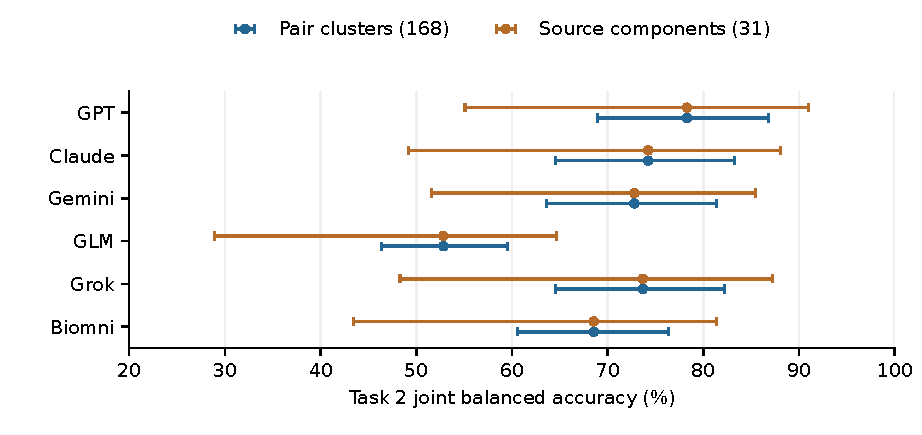
\includegraphics[width=.94\linewidth]{figs/cluster_intervals.pdf}
\caption{Task 2 joint balanced accuracy under two cluster assumptions. Dots show the unchanged published point estimate; bars are 95\% percentile intervals from 20,000 paired bootstrap draws. All units and four observed runs stay within the sampled cluster. Source components merge papers linked by shared pairs. Their wider intervals expose limited source diversity and do not incorporate judge uncertainty.}\label{fig:cluster_intervals}
\end{figure}
\begin{center}
\begin{tabular}{lrrrr}
\toprule
 & \multicolumn{2}{c}{Pair bootstrap} & \multicolumn{2}{c}{Source-component bootstrap} \\
System & Mean rank & First place (\%) & Mean rank & First place (\%) \\
\midrule
GPT & 1.02 & 97.97 & 1.13 & 88.54 \\
Claude & 2.58 & 1.98 & 2.84 & 6.79 \\
Gemini & 3.51 & 0.01 & 3.17 & 3.36 \\
GLM & 6.00 & 0.00 & 6.00 & 0.00 \\
Grok & 2.95 & 0.04 & 3.05 & 1.05 \\
Biomni & 4.94 & 0.00 & 4.81 & 0.25 \\
\bottomrule
\end{tabular}
\end{center}
Ties use midranks and split first-place credit. The entire original strict six-system ordering recurs in 36.35\% of pair draws and 18.96\% of source-component draws. GPT receives 97.97\% and 88.54\% of first-place credit. A comparatively frequent first place can coexist with uncertain adjacent ranks and a source-aware paired interval crossing zero. These frequencies describe this fixed benchmark, not the probability of a universal model ordering.

For the secondary equal-pair analysis, corrected tie-aware calculations retain the entire strict ordering in 52.76\% (chain) and 48.46\% (joint) of draws; mean Kendall $\tau_b$ is 0.924 and 0.921. Grok/Gemini invert in 28.70\% and 40.82\% of draws. Inversion counts compare the same systems in every draw, regardless of whether they remain adjacent. These calculations correct the supplied permutation-based rank comparison and adjacency-restricted flip counter without changing any pass-rate point estimate or interval.

\paragraph{Scope and reproducibility.} Per-pair dependence, source concentration, repeated-run variability and judge sensitivity are different uncertainty sources. This analysis addresses the first two while retaining observed runs; Appendix~\ref{app:judge_robustness} separately probes automated adjudication. Bootstrap intervals do not validate the biological labels or extrapolate to unseen TF families. The release includes source-component assignments, every bootstrap replicate, paired differences and all six-system rank summaries, together with deterministic reproduction scripts.
